%!TEX root = ./main.tex

\section{The model}

\begin{frame}{The model}

\alert{Goal}: given a set of $n$ data with $p$ variables, simultaneously infer the conditional dependence structure of such variables and their clustering.

\pause

\alert{Constraint}: the partition must respect the original order of the variables.
\pause
\begin{align*}
    \bm{y}_1, \ldots, \bm{y}_n \mid \bm{K} & \iid \mathcal{N}_p(\mathbf{0}, \bm{K}^{-1} ) \\
    \bm{K} \mid \bm{G} & \sim \GWish(b, D)\\
    P((i,j)&\in E\mid \bm{z},\bm{Q}) = Q_{z_{i} z_{j}},\quad \text{independent}\\
        Q_{rs} \mid \bm{z} &\ind \Beta(\alpha,\beta), \quad 1\leq r\leq s\leq M\\
    \bm{z} & \sim P\left(\bm{z}\right)
\end{align*}

The prior for the \alert{partition} $P(\bm{z})$ is (5) from \textcite{martinezNonparametricChangePoint2014}.

To improve the mixing of the chain, the two parameters of $P(\bm{z})$, namely $\theta$ and $\sigma$, are updated as in the original paper.

\end{frame}

\begin{frame}

$Q$ is marginalized out.
\pause

The prior for the \alert{graph} given the vector of group memberships is
\[
    P(\bm{G}\mid \bm{z})
    =
    \prod_{u=1}^{M}\prod_{v=u}^{M}
    \frac{B(\alpha + S_{uv}, \beta+ S^{\star}_{uv})}{B(\alpha,\beta)}
\]
where 
\begin{itemize}
    \item $S_{uv}$ is the sum of the edges between group $u$ and $v$.
    \item $S^{\star}_{uv}$ is the sum of the ``non-edges'', namely $S^{\star}_{uv} = T_{uv} - S_{uv}$ and $T_{uv}$ is the total number of possible edges.
\end{itemize}


\end{frame}


\section{Quick review of the sampling strategy}

\begin{frame}{Block Gibbs Sampler}
    Conditional distributions for our model:
    \begin{table}[tb]
        \centering
        \begin{tabular}{ll}
        \toprule
        Graph and Precision & $\small P(\bm{K},\bm{G} \mid \bm{Y},\bm{z}) \propto P(\bm{Y} \mid \bm{K})P(\bm{K} \mid \bm{G}) P(\bm{G} \mid \bm{z})$ \\
        \hline
        Random Partition & $\small P(\bm{z} \mid \bm{Y},\bm{K},\bm{G}) \propto P(\bm{Y} \mid \bm{K})P(\bm{K} \mid \bm{G})P(\bm{G} \mid \bm{z})P(\bm{z}) \propto P(\bm{G} \mid \bm{z})P(\bm{z}) $ \\
        \bottomrule
        \end{tabular}
    \end{table}

    \pause 

    We implement a block Gibbs sampling strategy:
    \begin{enumerate}
        \item \alert{Sampling Graph and Precision Matrix}\\
        $\bm{G}$ and $\bm{K}$ - given $\bm{z}$ - are sampled using a modified version of a Birth-and-Death chain (\cite{mohammadiBayesianStructureLearning2015a}), changing one link at a time. The modified Birth and Death rates take into account the dependency on the random partition.
        \item \alert{Sampling the Random Partition}\\
        Conditionally on $\bm{G}$, we can sample $\bm{z}$ through an adaptive split and merge sampler. \textcolor{white}{changepoints everywhere}
    \end{enumerate}
\end{frame}


\section{Simulations}

\begin{frame}{Simulations structure}
The Beta was reparametrized with mean and variance, with mean set to the graph density.

We ran a total of 41 simulations, varying different hyperparameters. 
Simulations divided into groups, depending on the parameter tuned:
    \begin{enumerate}
        \item Data generating \alert{seed}
        \item \alert{Variance} of the Beta prior \texttt{beta\_sig2}
        \item \alert{Initial partition} $\rho_0$
        \item Generating partition's \alert{cluster numerosities}
        \item Number of \alert{observations} $n$
        \item Number of \alert{nodes} $p$
        \item Using \alert{noised} block structure as data generator
    \end{enumerate}

\begin{table}[H]
\centering
\begin{tabular}{lllllll}
\cmidrule(l{3pt}r{3pt}){1-7} 
$n$ & $p$ & \texttt{data\_gen} & \texttt{seed} & $\bm{\rho}_0$ & \texttt{beta\_sig2} & $\bm{\rho}_{\text{true}}$ \\
\midrule
\end{tabular}
\end{table}
\end{frame}


\begin{frame}{Posterior analysis}

\begin{table}[h]
\centering
\begin{tabular}{llllll}
\cmidrule(l{1pt}r{1pt}){1-5}  %6
$\bm{\rho}_{\text{est}}$ & \texttt{accept} & VI & RI & KL \\ % & \texttt{time}\\
\midrule
\end{tabular}
\end{table}

    \begin{enumerate}
        \item $\bm{\rho}$ estimated by solving a minimization problem on the space of \emph{visited} partitions using  \alert{Variation of Information} (\alert{VI}) loss function
        \item Mean \alert{acceptance rate}
        \item \alert{Rand index} (\alert{RI}) used to measure the similarity between partitions
        \item \alert{Kullback-Leibler} (\alert{KL}) distance to compare generating and estimated precision matrices
    \end{enumerate}

        \pause

    The adjacency matrix estimated by taking the \alert{p-links} matrix (probability that a link is included in the graph) and choosing a threshold value $s$ using BFDR.

        %\item Plot of the estimated \emph{vs} generating \alert{precision matrix} 
        %\item Frequency barplot of how often a node was a splitting node
        %\item $\theta$ and $\sigma$ traceplot


\end{frame}


\begin{frame}{Theta and Sigma traceplots}

The traceplots of the prior parameters $\theta$ and $\sigma$ are similar throughout all the simulations.
\fg{0.75}{../../output/data/simulation_41/_theta_sigma_prior.pdf}
\textcolor{white}{A perfect mixing of the chain is to be appreciated.}

\end{frame}


\begin{frame}{Group 1: varying data generating seed}
\begin{table}[H]
\centering
\resizebox{\linewidth}{!}{
\begin{tabular}{lllllllllrrrrl}
\toprule
\multicolumn{1}{c}{ } & \multicolumn{7}{c}{Data} & \multicolumn{6}{c}{Analysis} \\
\cmidrule(l{3pt}r{3pt}){2-8} \cmidrule(l{3pt}r{3pt}){9-14}
\texttt{sim\_id} & $n$ & $p$ & \texttt{data\_gen} & \texttt{seed} & $\bm{\rho}_0$ & \texttt{beta\_sig2} & $\bm{\rho}_{\text{true}}$ & $\bm{\rho}_{\text{est}}$ & \texttt{accept} & VI & RI & KL & \texttt{time}\\
\midrule
\addlinespace[0.3em]
\cellcolor{gray!6}{\hspace{1em}01} & \cellcolor{gray!6}{500} & \cellcolor{gray!6}{25} & \cellcolor{gray!6}{BD} & \cellcolor{red!50}{22111996} & \cellcolor{gray!6}{25} & \cellcolor{gray!6}{0.2} & \cellcolor{gray!6}{8,4,8,5} & \cellcolor{gray!6}{8,4,8,5} & \cellcolor{gray!6}{0.019} & \cellcolor{gray!6}{0.017} & \cellcolor{gray!6}{1.000} & \cellcolor{gray!6}{0.187} & \cellcolor{gray!6}{1.21400 mins}\\
\cellcolor{gray!6}{\hspace{1em}02} & \cellcolor{gray!6}{500} & \cellcolor{gray!6}{25} & \cellcolor{gray!6}{BD} & \cellcolor{red!50}{31051999} & \cellcolor{gray!6}{25} & \cellcolor{gray!6}{0.2} & \cellcolor{gray!6}{8,4,8,5} & \cellcolor{gray!6}{8,4,8,5} & \cellcolor{gray!6}{0.019} & \cellcolor{gray!6}{0.017} & \cellcolor{gray!6}{1.000} & \cellcolor{gray!6}{0.187} & \cellcolor{gray!6}{1.21800 mins}\\
\cellcolor{gray!6}{\hspace{1em}03} & \cellcolor{gray!6}{500} & \cellcolor{gray!6}{25} & \cellcolor{gray!6}{BD} & \cellcolor{red!50}{27051999} & \cellcolor{gray!6}{25} & \cellcolor{gray!6}{0.2} & \cellcolor{gray!6}{8,4,8,5} & \cellcolor{gray!6}{8,4,8,5} & \cellcolor{gray!6}{0.019} & \cellcolor{gray!6}{0.017} & \cellcolor{gray!6}{1.000} & \cellcolor{gray!6}{0.187} & \cellcolor{gray!6}{1.21700 mins}\\
\cellcolor{gray!6}{\hspace{1em}04} & \cellcolor{gray!6}{500} & \cellcolor{gray!6}{25} & \cellcolor{gray!6}{BD} & \cellcolor{red!50}{29061999} & \cellcolor{gray!6}{25} & \cellcolor{gray!6}{0.2} & \cellcolor{gray!6}{8,4,8,5} & \cellcolor{gray!6}{8,4,8,5} & \cellcolor{gray!6}{0.019} & \cellcolor{gray!6}{0.017} & \cellcolor{gray!6}{1.000} & \cellcolor{gray!6}{0.187} & \cellcolor{gray!6}{1.21700 mins}\\
\cellcolor{gray!6}{\hspace{1em}05} & \cellcolor{gray!6}{500} & \cellcolor{gray!6}{25} & \cellcolor{gray!6}{BD} & \cellcolor{red!50}{12091997} & \cellcolor{gray!6}{25} & \cellcolor{gray!6}{0.2} & \cellcolor{gray!6}{8,4,8,5} & \cellcolor{gray!6}{8,4,8,5} & \cellcolor{gray!6}{0.019} & \cellcolor{gray!6}{0.017} & \cellcolor{gray!6}{1.000} & \cellcolor{gray!6}{0.187} & \cellcolor{gray!6}{1.21600 mins}\\
\cellcolor{gray!6}{\hspace{1em}06} & \cellcolor{gray!6}{500} & \cellcolor{gray!6}{25} & \cellcolor{gray!6}{BD} & \cellcolor{red!50}{27091999} & \cellcolor{gray!6}{25} & \cellcolor{gray!6}{0.2} & \cellcolor{gray!6}{8,4,8,5} & \cellcolor{gray!6}{8,4,8,5} & \cellcolor{gray!6}{0.019} & \cellcolor{gray!6}{0.017} & \cellcolor{gray!6}{1.000} & \cellcolor{gray!6}{0.187} & \cellcolor{gray!6}{1.21500 mins}\\
\cellcolor{gray!6}{\hspace{1em}07} & \cellcolor{gray!6}{500} & \cellcolor{gray!6}{25} & \cellcolor{gray!6}{BD} & \cellcolor{red!50}{27121996} & \cellcolor{gray!6}{25} & \cellcolor{gray!6}{0.2} & \cellcolor{gray!6}{8,4,8,5} & \cellcolor{gray!6}{8,4,8,5} & \cellcolor{gray!6}{0.019} & \cellcolor{gray!6}{0.017} & \cellcolor{gray!6}{1.000} & \cellcolor{gray!6}{0.187} & \cellcolor{gray!6}{1.21700 mins}\\
\bottomrule
\end{tabular}}
\end{table}

Results are consistent for every seed:
\begin{itemize}
    \item Estimated partition coincides with the generating partition (RI=1)
    \item KL distance converges to 0.187
    \item Estimated adjacency matrix is close to the generating adjacency matrix

\end{itemize}
\end{frame}




\begin{frame}{Group 1: varying data generating seed}
\begin{table}[H]
\centering
\resizebox{\linewidth}{!}{
\begin{tabular}{lllllllllrrrrl}
\toprule
\cmidrule(l{3pt}r{3pt}){2-8} \cmidrule(l{3pt}r{3pt}){9-14}
\texttt{sim\_id} & $n$ & $p$ & \texttt{data\_gen} & \texttt{seed} & $\bm{\rho}_0$ & \texttt{beta\_sig2} & $\bm{\rho}_{\text{true}}$ & $\bm{\rho}_{\text{est}}$ & \texttt{accept} & VI & RI & KL & \texttt{time}\\
\midrule
\addlinespace[0.3em]
\cellcolor{gray!6}{\hspace{1em}02} & \cellcolor{gray!6}{500} & \cellcolor{gray!6}{25} & \cellcolor{gray!6}{BD} & \cellcolor{gray!6}{31051999} & \cellcolor{gray!6}{25} & \cellcolor{gray!6}{0.2} & \cellcolor{gray!6}{8,4,8,5} & \cellcolor{gray!6}{8,4,8,5} & \cellcolor{gray!6}{0.019} & \cellcolor{gray!6}{0.017} & \cellcolor{gray!6}{1.000} & \cellcolor{gray!6}{0.187} & \cellcolor{gray!6}{1.21800 mins}\\
\bottomrule
\end{tabular}}
\end{table}
\begin{figure}
\begin{minipage}[c]{0.49\linewidth}
\fg{1.05}{../../output/data/simulation_02/comparison_G_true_est.pdf}
\end{minipage}
\hfill
\begin{minipage}[c]{0.49\linewidth}
\fg{1.05}{../../output/data/simulation_02/comparison_K_true_est.pdf}
\end{minipage}%
\end{figure}
\end{frame}




\begin{frame}{Group 1: varying data generating seed}
\begin{table}[H]
\centering
\resizebox{\linewidth}{!}{
\begin{tabular}{lllllllllrrrrl}
\toprule
\cmidrule(l{3pt}r{3pt}){2-8} \cmidrule(l{3pt}r{3pt}){9-14}
\texttt{sim\_id} & $n$ & $p$ & \texttt{data\_gen} & \texttt{seed} & $\bm{\rho}_0$ & \texttt{beta\_sig2} & $\bm{\rho}_{\text{true}}$ & $\bm{\rho}_{\text{est}}$ & \texttt{accept} & VI & RI & KL & \texttt{time}\\
\midrule
\addlinespace[0.3em]
\cellcolor{gray!6}{\hspace{1em}02} & \cellcolor{gray!6}{500} & \cellcolor{gray!6}{25} & \cellcolor{gray!6}{BD} & \cellcolor{gray!6}{31051999} & \cellcolor{gray!6}{25} & \cellcolor{gray!6}{0.2} & \cellcolor{gray!6}{8,4,8,5} & \cellcolor{gray!6}{8,4,8,5} & \cellcolor{gray!6}{0.019} & \cellcolor{gray!6}{0.017} & \cellcolor{gray!6}{1.000} & \cellcolor{gray!6}{0.187} & \cellcolor{gray!6}{1.21800 mins}\\
\bottomrule
\end{tabular}}
\end{table}
\fg{0.65}{../../output/data/simulation_02/graph.pdf}
\end{frame}


\begin{frame}{Group 1: varying data generating seed}
\begin{table}[H]
\centering
\resizebox{\linewidth}{!}{
\begin{tabular}{lllllllllrrrrl}
\toprule
\cmidrule(l{3pt}r{3pt}){2-8} \cmidrule(l{3pt}r{3pt}){9-14}
\texttt{sim\_id} & $n$ & $p$ & \texttt{data\_gen} & \texttt{seed} & $\bm{\rho}_0$ & \texttt{beta\_sig2} & $\bm{\rho}_{\text{true}}$ & $\bm{\rho}_{\text{est}}$ & \texttt{accept} & VI & RI & KL & \texttt{time}\\
\midrule
\addlinespace[0.3em]
\cellcolor{gray!6}{\hspace{1em}02} & \cellcolor{gray!6}{500} & \cellcolor{gray!6}{25} & \cellcolor{gray!6}{BD} & \cellcolor{gray!6}{31051999} & \cellcolor{gray!6}{25} & \cellcolor{gray!6}{0.2} & \cellcolor{gray!6}{8,4,8,5} & \cellcolor{gray!6}{8,4,8,5} & \cellcolor{gray!6}{0.019} & \cellcolor{gray!6}{0.017} & \cellcolor{gray!6}{1.000} & \cellcolor{gray!6}{0.187} & \cellcolor{gray!6}{1.21800 mins}\\
\bottomrule
\end{tabular}}
\end{table}
\fg{1}{../../output/data/simulation_02/indexes.pdf}
\end{frame}




\begin{frame}{Group 2: Changing the variance of the Beta prior}
\begin{table}[H]
\centering
\resizebox{\linewidth}{!}{
\begin{tabular}{lllllllllrrrrl}
\toprule
\multicolumn{1}{c}{ } & \multicolumn{7}{c}{Data} & \multicolumn{6}{c}{Analysis} \\
\cmidrule(l{3pt}r{3pt}){2-8} \cmidrule(l{3pt}r{3pt}){9-14}
\texttt{sim\_id} & $n$ & $p$ & \texttt{data\_gen} & \texttt{seed} & $\bm{\rho}_0$ & \texttt{beta\_sig2} & $\bm{\rho}_{\text{true}}$ & $\bm{\rho}_{\text{est}}$ & \texttt{accept} & VI & RI & KL & \texttt{time}\\
\midrule
\addlinespace[0.3em]
\cellcolor{gray!6}{\hspace{1em}08} & \cellcolor{gray!6}{500} & \cellcolor{gray!6}{25} & \cellcolor{gray!6}{BD} & \cellcolor{gray!6}{27121996} & \cellcolor{gray!6}{25} & \cellcolor{red!50}{0.062} & \cellcolor{gray!6}{8,4,8,5} & \cellcolor{gray!6}{8,4,8,5} & \cellcolor{gray!6}{0.066} & \cellcolor{gray!6}{0.034} & \cellcolor{gray!6}{1.000} & \cellcolor{gray!6}{0.191} & \cellcolor{gray!6}{1.22400 mins}\\
\cellcolor{gray!6}{\hspace{1em}09} & \cellcolor{gray!6}{500} & \cellcolor{gray!6}{25} & \cellcolor{gray!6}{BD} & \cellcolor{gray!6}{27121996} & \cellcolor{gray!6}{25} & \cellcolor{red!50}{0.078} & \cellcolor{gray!6}{8,4,8,5} & \cellcolor{gray!6}{8,4,8,5} & \cellcolor{gray!6}{0.080} & \cellcolor{gray!6}{0.043} & \cellcolor{gray!6}{1.000} & \cellcolor{gray!6}{0.186} & \cellcolor{gray!6}{1.20700 mins}\\
\cellcolor{gray!6}{\hspace{1em}10} & \cellcolor{gray!6}{500} & \cellcolor{gray!6}{25} & \cellcolor{gray!6}{BD} & \cellcolor{gray!6}{27121996} & \cellcolor{gray!6}{25} & \cellcolor{red!50}{0.093} & \cellcolor{gray!6}{8,4,8,5} & \cellcolor{gray!6}{8,4,8,5} & \cellcolor{gray!6}{0.075} & \cellcolor{gray!6}{0.039} & \cellcolor{gray!6}{1.000} & \cellcolor{gray!6}{0.188} & \cellcolor{gray!6}{1.20600 mins}\\
\cellcolor{gray!6}{\hspace{1em}11} & \cellcolor{gray!6}{500} & \cellcolor{gray!6}{25} & \cellcolor{gray!6}{BD} & \cellcolor{gray!6}{27121996} & \cellcolor{gray!6}{25} & \cellcolor{red!50}{0.108} & \cellcolor{gray!6}{8,4,8,5} & \cellcolor{gray!6}{8,4,8,5} & \cellcolor{gray!6}{0.079} & \cellcolor{gray!6}{0.049} & \cellcolor{gray!6}{1.000} & \cellcolor{gray!6}{0.188} & \cellcolor{gray!6}{1.20800 mins}\\
\cellcolor{gray!6}{\hspace{1em}12} & \cellcolor{gray!6}{500} & \cellcolor{gray!6}{25} & \cellcolor{gray!6}{BD} & \cellcolor{gray!6}{27121996} & \cellcolor{gray!6}{25} & \cellcolor{red!50}{0.124} & \cellcolor{gray!6}{8,4,8,5} & \cellcolor{gray!6}{8,4,8,5} & \cellcolor{gray!6}{0.067} & \cellcolor{gray!6}{0.040} & \cellcolor{gray!6}{1.000} & \cellcolor{gray!6}{0.188} & \cellcolor{gray!6}{1.20100 mins}\\
\cellcolor{gray!6}{\hspace{1em}13} & \cellcolor{gray!6}{500} & \cellcolor{gray!6}{25} & \cellcolor{gray!6}{BD} & \cellcolor{gray!6}{27121996} & \cellcolor{gray!6}{25} & \cellcolor{red!50}{0.139} & \cellcolor{gray!6}{8,4,8,5} & \cellcolor{gray!6}{8,4,8,5} & \cellcolor{gray!6}{0.060} & \cellcolor{gray!6}{0.035} & \cellcolor{gray!6}{1.000} & \cellcolor{gray!6}{0.188} & \cellcolor{gray!6}{1.20200 mins}\\
\cellcolor{gray!6}{\hspace{1em}14} & \cellcolor{gray!6}{500} & \cellcolor{gray!6}{25} & \cellcolor{gray!6}{BD} & \cellcolor{gray!6}{27121996} & \cellcolor{gray!6}{25} & \cellcolor{red!50}{0.154} & \cellcolor{gray!6}{8,4,8,5} & \cellcolor{gray!6}{8,4,8,5} & \cellcolor{gray!6}{0.056} & \cellcolor{gray!6}{0.030} & \cellcolor{gray!6}{1.000} & \cellcolor{gray!6}{0.193} & \cellcolor{gray!6}{1.20000 mins}\\
\cellcolor{gray!6}{\hspace{1em}15} & \cellcolor{gray!6}{500} & \cellcolor{gray!6}{25} & \cellcolor{gray!6}{BD} & \cellcolor{gray!6}{27121996} & \cellcolor{gray!6}{25} & \cellcolor{red!50}{0.169} & \cellcolor{gray!6}{8,4,8,5} & \cellcolor{gray!6}{8,4,8,5} & \cellcolor{gray!6}{0.047} & \cellcolor{gray!6}{0.024} & \cellcolor{gray!6}{1.000} & \cellcolor{gray!6}{0.191} & \cellcolor{gray!6}{1.20100 mins}\\
\cellcolor{gray!6}{\hspace{1em}16} & \cellcolor{gray!6}{500} & \cellcolor{gray!6}{25} & \cellcolor{gray!6}{BD} & \cellcolor{gray!6}{27121996} & \cellcolor{gray!6}{25} & \cellcolor{red!50}{0.185} & \cellcolor{gray!6}{8,4,8,5} & \cellcolor{gray!6}{8,4,8,5} & \cellcolor{gray!6}{0.034} & \cellcolor{gray!6}{0.022} & \cellcolor{gray!6}{1.000} & \cellcolor{gray!6}{0.189} & \cellcolor{gray!6}{1.20000 mins}\\
\cellcolor{gray!6}{\hspace{1em}17} & \cellcolor{gray!6}{500} & \cellcolor{gray!6}{25} & \cellcolor{gray!6}{BD} & \cellcolor{gray!6}{27121996} & \cellcolor{gray!6}{25} & \cellcolor{red!50}{0.2} & \cellcolor{gray!6}{8,4,8,5} & \cellcolor{gray!6}{8,4,8,5} & \cellcolor{gray!6}{0.019} & \cellcolor{gray!6}{0.017} & \cellcolor{gray!6}{1.000} & \cellcolor{gray!6}{0.187} & \cellcolor{gray!6}{1.16200 mins}\\
\bottomrule
\end{tabular}}
\end{table}

Changing the \alert{variance of the Beta prior} does not yield significant changes in posterior analysis.

\end{frame}


\begin{frame}{Group 2: Changing the variance of the beta prior}
\fg{0.8}{../../output/kl_dist_comparison_beta_sig2-1.pdf}

\end{frame}


\begin{frame}{Group 3: VARYING INITIAL PARTITION}
\begin{table}[H]
\centering
\resizebox{\linewidth}{!}{
\begin{tabular}{lllllllllrrrrl}
\toprule
\multicolumn{1}{c}{ } & \multicolumn{7}{c}{Data} & \multicolumn{6}{c}{Analysis} \\
\cmidrule(l{3pt}r{3pt}){2-8} \cmidrule(l{3pt}r{3pt}){9-14}
\texttt{sim\_id} & $n$ & $p$ & \texttt{data\_gen} & \texttt{seed} & $\bm{\rho}_0$ & \texttt{beta\_sig2} & $\bm{\rho}_{\text{true}}$ & $\bm{\rho}_{\text{est}}$ & \texttt{accept} & VI & RI & KL & \texttt{time}\\
\midrule
\addlinespace[0.3em]
\cellcolor{gray!6}{\hspace{1em}18} & \cellcolor{gray!6}{500} & \cellcolor{gray!6}{25} & \cellcolor{gray!6}{BD} & \cellcolor{gray!6}{27121996} & \cellcolor{red!50}{25} & \cellcolor{gray!6}{0.2} & \cellcolor{gray!6}{8,4,8,5} & \cellcolor{gray!6}{8,4,8,5} & \cellcolor{gray!6}{0.019} & \cellcolor{gray!6}{0.017} & \cellcolor{gray!6}{1.000} & \cellcolor{gray!6}{0.187} & \cellcolor{gray!6}{1.16300 mins}\\
\cellcolor{gray!6}{\hspace{1em}19} & \cellcolor{gray!6}{500} & \cellcolor{gray!6}{25} & \cellcolor{gray!6}{BD} & \cellcolor{gray!6}{27121996} & \cellcolor{red!50}{singletons} & \cellcolor{gray!6}{0.2} & \cellcolor{gray!6}{8,4,8,5} & \cellcolor{gray!6}{8,4,8,5} & \cellcolor{gray!6}{0.020} & \cellcolor{gray!6}{0.015} & \cellcolor{gray!6}{1.000} & \cellcolor{gray!6}{0.189} & \cellcolor{gray!6}{1.24800 mins}\\
\bottomrule
\end{tabular}}
\end{table}

Starting from different initial partitions (i.e. one single partition or all singletons) does not affect the final result.

\end{frame}





\begin{frame}{Group 4: VARYING GENERATING PARTITION'S CLUSTER NUMEROSITIES}
\begin{table}[H]
\centering
\resizebox{\linewidth}{!}{
\begin{tabular}{lllllllllrrrrl}
\toprule
\multicolumn{1}{c}{ } & \multicolumn{7}{c}{Data} & \multicolumn{6}{c}{Analysis} \\
\cmidrule(l{3pt}r{3pt}){2-8} \cmidrule(l{3pt}r{3pt}){9-14}
\texttt{sim\_id} & $n$ & $p$ & \texttt{data\_gen} & \texttt{seed} & $\bm{\rho}_0$ & \texttt{beta\_sig2} & $\bm{\rho}_{\text{true}}$ & $\bm{\rho}_{\text{est}}$ & \texttt{accept} & VI & RI & KL & \texttt{time}\\
\midrule
\addlinespace[0.3em]
\cellcolor{gray!6}{\hspace{1em}20} & \cellcolor{gray!6}{500} & \cellcolor{gray!6}{25} & \cellcolor{gray!6}{BD} & \cellcolor{gray!6}{27121996} & \cellcolor{gray!6}{25} & \cellcolor{gray!6}{0.2} & \cellcolor{red!50}{8,4,8,5} & \cellcolor{gray!6}{8,4,8,5} & \cellcolor{gray!6}{0.019} & \cellcolor{gray!6}{0.017} & \cellcolor{gray!6}{1.000} & \cellcolor{gray!6}{0.187} & \cellcolor{gray!6}{1.16000 mins}\\
\cellcolor{gray!6}{\hspace{1em}21} & \cellcolor{gray!6}{500} & \cellcolor{gray!6}{25} & \cellcolor{gray!6}{BD} & \cellcolor{gray!6}{27121996} & \cellcolor{gray!6}{25} & \cellcolor{gray!6}{0.2} & \cellcolor{red!50}{1,10,2,9,3} & \cellcolor{gray!6}{1,10,2,9,3} & \cellcolor{gray!6}{0.072} & \cellcolor{gray!6}{0.109} & \cellcolor{gray!6}{1.000} & \cellcolor{gray!6}{0.181} & \cellcolor{gray!6}{1.25500 mins}\\
\cellcolor{gray!6}{\hspace{1em}22} & \cellcolor{gray!6}{500} & \cellcolor{gray!6}{25} & \cellcolor{gray!6}{BD} & \cellcolor{gray!6}{27121996} & \cellcolor{gray!6}{25} & \cellcolor{gray!6}{0.02} & \cellcolor{red!50}{1,3,2,4,2,3,3,4,3} & \cellcolor{gray!6}{18,7} & \cellcolor{gray!6}{0.397} & \cellcolor{gray!6}{1.020} & \cellcolor{gray!6}{0.129} & \cellcolor{gray!6}{0.126} & \cellcolor{gray!6}{1.10700 mins}\\
\cellcolor{gray!6}{\hspace{1em}23} & \cellcolor{gray!6}{500} & \cellcolor{gray!6}{25} & \cellcolor{gray!6}{BD} & \cellcolor{gray!6}{27121996} & \cellcolor{gray!6}{25} & \cellcolor{gray!6}{0.2} & \cellcolor{red!50}{12,13} & \cellcolor{gray!6}{12,13} & \cellcolor{gray!6}{0.129} & \cellcolor{gray!6}{0.073} & \cellcolor{gray!6}{1.000} & \cellcolor{gray!6}{0.255} & \cellcolor{gray!6}{1.36700 mins}\\
\bottomrule
\end{tabular}}
\end{table}

Changing the generating partition's cluster numerosities does not generally influence the result. The only exception comes with small and numerous clusters, as in simulation 22.

Let's have a closer look.
\end{frame}




\begin{frame}{Group 4: VARYING GENERATING PARTITION'S CLUSTER NUMEROSITIES}
\begin{table}[H]
\centering
\resizebox{\linewidth}{!}{
\begin{tabular}{lllllllllrrrrl}
\toprule
\multicolumn{1}{c}{ } & \multicolumn{7}{c}{Data} & \multicolumn{6}{c}{Analysis} \\
\cmidrule(l{3pt}r{3pt}){2-8} \cmidrule(l{3pt}r{3pt}){9-14}
\texttt{sim\_id} & $n$ & $p$ & \texttt{data\_gen} & \texttt{seed} & $\bm{\rho}_0$ & \texttt{beta\_sig2} & $\bm{\rho}_{\text{true}}$ & $\bm{\rho}_{\text{est}}$ & \texttt{accept} & VI & RI & KL & \texttt{time}\\
\midrule
\addlinespace[0.3em]
\cellcolor{gray!6}{\hspace{1em}22} & \cellcolor{gray!6}{500} & \cellcolor{gray!6}{25} & \cellcolor{gray!6}{BD} & \cellcolor{gray!6}{27121996} & \cellcolor{gray!6}{25} & \cellcolor{gray!6}{0.02} & \cellcolor{red!50}{1,3,2,4,2,3,3,4,3} & \cellcolor{blue!50}{18,7} & \cellcolor{gray!6}{0.397} & \cellcolor{gray!6}{1.020} & \cellcolor{gray!6}{0.129} & \cellcolor{gray!6}{0.126} & \cellcolor{gray!6}{1.10700 mins}\\
\bottomrule
\end{tabular}}
\end{table}

\begin{figure}
\begin{minipage}[c]{0.49\linewidth}
\fg{1.05}{../../output/data/simulation_22/comparison_G_true_est.pdf}
\end{minipage}
\hfill
\begin{minipage}[c]{0.49\linewidth}
\fg{1.05}{../../output/data/simulation_22/comparison_K_true_est.pdf}
\end{minipage}%
\end{figure}
\end{frame}






\begin{frame}{Group 4: VARYING GENERATING PARTITION'S CLUSTER NUMEROSITIES}
\begin{table}[H]
\centering
\resizebox{\linewidth}{!}{
\begin{tabular}{lllllllllrrrrl}
\toprule
\multicolumn{1}{c}{ } & \multicolumn{7}{c}{Data} & \multicolumn{6}{c}{Analysis} \\
\cmidrule(l{3pt}r{3pt}){2-8} \cmidrule(l{3pt}r{3pt}){9-14}
\texttt{sim\_id} & $n$ & $p$ & \texttt{data\_gen} & \texttt{seed} & $\bm{\rho}_0$ & \texttt{beta\_sig2} & $\bm{\rho}_{\text{true}}$ & $\bm{\rho}_{\text{est}}$ & \texttt{accept} & VI & RI & KL & \texttt{time}\\
\midrule
\addlinespace[0.3em]
\cellcolor{gray!6}{\hspace{1em}22} & \cellcolor{gray!6}{500} & \cellcolor{gray!6}{25} & \cellcolor{gray!6}{BD} & \cellcolor{gray!6}{27121996} & \cellcolor{gray!6}{25} & \cellcolor{gray!6}{0.02} & \cellcolor{red!50}{1,3,2,4,2,3,3,4,3} & \cellcolor{blue!50}{18,7} & \cellcolor{gray!6}{0.397} & \cellcolor{gray!6}{1.020} & \cellcolor{gray!6}{0.129} & \cellcolor{gray!6}{0.126} & \cellcolor{gray!6}{1.10700 mins}\\
\bottomrule
\end{tabular}}
\end{table}
The result is actually not so bad, possible criteria improvement.
\fg{0.8}{../../output/data/simulation_22/indexes.pdf}

\end{frame}







\begin{frame}{Group 5: varying number of observations}
\begin{table}[H]
\centering
\resizebox{\linewidth}{!}{
\begin{tabular}{lllllllllrrrrl}
\toprule
\multicolumn{1}{c}{ } & \multicolumn{7}{c}{Data} & \multicolumn{6}{c}{Analysis} \\
\cmidrule(l{3pt}r{3pt}){2-8} \cmidrule(l{3pt}r{3pt}){9-14}
\texttt{sim\_id} & $n$ & $p$ & \texttt{data\_gen} & \texttt{seed} & $\bm{\rho}_0$ & \texttt{beta\_sig2} & $\bm{\rho}_{\text{true}}$ & $\bm{\rho}_{\text{est}}$ & \texttt{accept} & VI & RI & KL & \texttt{time}\\
\midrule
\addlinespace[0.3em]
\cellcolor{gray!6}{\hspace{1em}24} & \cellcolor{red!50}{500} & \cellcolor{gray!6}{25} & \cellcolor{gray!6}{BD} & \cellcolor{gray!6}{27121996} & \cellcolor{gray!6}{25} & \cellcolor{gray!6}{0.1} & \cellcolor{gray!6}{8,4,8,5} & \cellcolor{gray!6}{8,4,8,5} & \cellcolor{gray!6}{0.082} & \cellcolor{gray!6}{0.046} & \cellcolor{gray!6}{1.000} & \cellcolor{gray!6}{0.187} & \cellcolor{gray!6}{1.17300 mins}\\
\cellcolor{gray!6}{\hspace{1em}25} & \cellcolor{red!50}{400} & \cellcolor{gray!6}{25} & \cellcolor{gray!6}{BD} & \cellcolor{gray!6}{27121996} & \cellcolor{gray!6}{25} & \cellcolor{gray!6}{0.1} & \cellcolor{gray!6}{8,4,8,5} & \cellcolor{gray!6}{8,4,8,5} & \cellcolor{gray!6}{0.072} & \cellcolor{gray!6}{0.036} & \cellcolor{gray!6}{1.000} & \cellcolor{gray!6}{0.221} & \cellcolor{gray!6}{1.15900 mins}\\
\cellcolor{gray!6}{\hspace{1em}26} & \cellcolor{red!50}{300} & \cellcolor{gray!6}{25} & \cellcolor{gray!6}{BD} & \cellcolor{gray!6}{27121996} & \cellcolor{gray!6}{25} & \cellcolor{gray!6}{0.1} & \cellcolor{gray!6}{8,4,8,5} & \cellcolor{gray!6}{8,4,8,5} & \cellcolor{gray!6}{0.070} & \cellcolor{gray!6}{0.041} & \cellcolor{gray!6}{1.000} & \cellcolor{gray!6}{0.336} & \cellcolor{gray!6}{1.16800 mins}\\
\cellcolor{gray!6}{\hspace{1em}27} & \cellcolor{red!50}{200} & \cellcolor{gray!6}{25} & \cellcolor{gray!6}{BD} & \cellcolor{gray!6}{27121996} & \cellcolor{gray!6}{25} & \cellcolor{gray!6}{0.1} & \cellcolor{gray!6}{8,4,8,5} & \cellcolor{gray!6}{8,4,8,5} & \cellcolor{gray!6}{0.074} & \cellcolor{gray!6}{0.045} & \cellcolor{gray!6}{1.000} & \cellcolor{gray!6}{0.532} & \cellcolor{gray!6}{1.15400 mins}\\
\cellcolor{gray!6}{\hspace{1em}28} & \cellcolor{red!50}{100} & \cellcolor{gray!6}{25} & \cellcolor{gray!6}{BD} & \cellcolor{gray!6}{27121996} & \cellcolor{gray!6}{25} & \cellcolor{gray!6}{0.1} & \cellcolor{gray!6}{8,4,8,5} & \cellcolor{gray!6}{8,4,8,5} & \cellcolor{gray!6}{0.111} & \cellcolor{gray!6}{0.241} & \cellcolor{gray!6}{1.000} & \cellcolor{gray!6}{1.487} & \cellcolor{gray!6}{1.11800 mins}\\
\cellcolor{gray!6}{\hspace{1em}29} & \cellcolor{red!50}{50} & \cellcolor{gray!6}{25} & \cellcolor{gray!6}{BD} & \cellcolor{gray!6}{27121996} & \cellcolor{gray!6}{25} & \cellcolor{gray!6}{0.1} & \cellcolor{gray!6}{8,4,8,5} & \cellcolor{gray!6}{20,5} & \cellcolor{gray!6}{0.236} & \cellcolor{gray!6}{0.539} & \cellcolor{gray!6}{0.273} & \cellcolor{gray!6}{4.212} & \cellcolor{gray!6}{1.09000 mins}\\
\cellcolor{gray!6}{\hspace{1em}30} & \cellcolor{red!50}{20} & \cellcolor{gray!6}{25} & \cellcolor{gray!6}{BD} & \cellcolor{gray!6}{27121996} & \cellcolor{gray!6}{25} & \cellcolor{gray!6}{0.1} & \cellcolor{gray!6}{8,4,8,5} & \cellcolor{gray!6}{25} & \cellcolor{gray!6}{0.280} & \cellcolor{gray!6}{0.241} & \cellcolor{gray!6}{0.000} & \cellcolor{gray!6}{11.854} & \cellcolor{gray!6}{1.07600 mins}\\
\bottomrule
\end{tabular}}
\end{table}

As $n$ diminishes and becomes comparable to $p$, we notice that the KL distance plateaus on progressively higher values, and VI and RI behave accordingly.
The acceptance rates rises in \textit{more difficult} situations.
\end{frame}





\begin{frame}{Group 5: varying number of observations}
\fg{0.8}{../../output/kl_dist_comparison_n-1.pdf}
\end{frame}






\begin{frame}{Group 6: VARYING NUMBER OF NODES}
\begin{table}[H]
\centering
\resizebox{\linewidth}{!}{
\begin{tabular}{lllllllllrrrrl}
\toprule
\multicolumn{1}{c}{ } & \multicolumn{7}{c}{Data} & \multicolumn{6}{c}{Analysis} \\
\cmidrule(l{3pt}r{3pt}){2-8} \cmidrule(l{3pt}r{3pt}){9-14}
\texttt{sim\_id} & $n$ & $p$ & \texttt{data\_gen} & \texttt{seed} & $\bm{\rho}_0$ & \texttt{beta\_sig2} & $\bm{\rho}_{\text{true}}$ & $\bm{\rho}_{\text{est}}$ & \texttt{accept} & VI & RI & KL & \texttt{time}\\
\midrule
\addlinespace[0.3em]
\cellcolor{gray!6}{\hspace{1em}31} & \cellcolor{gray!6}{500} & \cellcolor{red!50}{5} & \cellcolor{gray!6}{BD} & \cellcolor{gray!6}{27121996} & \cellcolor{gray!6}{5} & \cellcolor{gray!6}{0.0625} & \cellcolor{gray!6}{3,2} & \cellcolor{gray!6}{3,2} & \cellcolor{gray!6}{0.543} & \cellcolor{gray!6}{0.752} & \cellcolor{gray!6}{1.000} & \cellcolor{gray!6}{0.006} & \cellcolor{gray!6}{0.79960 mins}\\
\cellcolor{gray!6}{\hspace{1em}32} & \cellcolor{gray!6}{500} & \cellcolor{red!50}{10} & \cellcolor{gray!6}{BD} & \cellcolor{gray!6}{27121996} & \cellcolor{gray!6}{10} & \cellcolor{gray!6}{0.0625} & \cellcolor{gray!6}{5,5} & \cellcolor{gray!6}{5,5} & \cellcolor{gray!6}{0.188} & \cellcolor{gray!6}{0.115} & \cellcolor{gray!6}{1.000} & \cellcolor{gray!6}{0.028} & \cellcolor{gray!6}{0.85055 mins}\\
\cellcolor{gray!6}{\hspace{1em}33} & \cellcolor{gray!6}{500} & \cellcolor{red!50}{15} & \cellcolor{gray!6}{BD} & \cellcolor{gray!6}{27121996} & \cellcolor{gray!6}{15} & \cellcolor{gray!6}{0.0625} & \cellcolor{gray!6}{5,5,5} & \cellcolor{gray!6}{5,5,5} & \cellcolor{gray!6}{0.129} & \cellcolor{gray!6}{0.087} & \cellcolor{gray!6}{1.000} & \cellcolor{gray!6}{0.045} & \cellcolor{gray!6}{1.09400 mins}\\
\cellcolor{gray!6}{\hspace{1em}34} & \cellcolor{gray!6}{500} & \cellcolor{red!50}{20} & \cellcolor{gray!6}{BD} & \cellcolor{gray!6}{27121996} & \cellcolor{gray!6}{20} & \cellcolor{gray!6}{0.0625} & \cellcolor{gray!6}{5,5,5,5} & \cellcolor{gray!6}{5,5,5,5} & \cellcolor{gray!6}{0.103} & \cellcolor{gray!6}{0.070} & \cellcolor{gray!6}{1.000} & \cellcolor{gray!6}{0.118} & \cellcolor{gray!6}{1.20100 mins}\\
\cellcolor{gray!6}{\hspace{1em}35} & \cellcolor{gray!6}{500} & \cellcolor{red!50}{25} & \cellcolor{gray!6}{BD} & \cellcolor{gray!6}{27121996} & \cellcolor{gray!6}{25} & \cellcolor{gray!6}{0.0625} & \cellcolor{gray!6}{5,5,5,5,5} & \cellcolor{gray!6}{5,5,5,5,5} & \cellcolor{gray!6}{0.104} & \cellcolor{gray!6}{0.074} & \cellcolor{gray!6}{1.000} & \cellcolor{gray!6}{0.170} & \cellcolor{gray!6}{1.33600 mins}\\
\cellcolor{gray!6}{\hspace{1em}36} & \cellcolor{gray!6}{500} & \cellcolor{red!50}{30} & \cellcolor{gray!6}{BD} & \cellcolor{gray!6}{27121996} & \cellcolor{gray!6}{30} & \cellcolor{gray!6}{0.0625} & \cellcolor{gray!6}{5,5,5,5,5,5} & \cellcolor{gray!6}{5,5,5,5,5,5} & \cellcolor{gray!6}{0.080} & \cellcolor{gray!6}{0.061} & \cellcolor{gray!6}{1.000} & \cellcolor{gray!6}{0.140} & \cellcolor{gray!6}{1.49600 mins}\\
\cellcolor{gray!6}{\hspace{1em}37} & \cellcolor{gray!6}{500} & \cellcolor{red!50}{35} & \cellcolor{gray!6}{BD} & \cellcolor{gray!6}{27121996} & \cellcolor{gray!6}{35} & \cellcolor{gray!6}{0.0625} & \cellcolor{gray!6}{5,5,5,5,5,5,5} & \cellcolor{gray!6}{5,5,5,5,5,5,5} & \cellcolor{gray!6}{0.066} & \cellcolor{gray!6}{0.149} & \cellcolor{gray!6}{1.000} & \cellcolor{gray!6}{0.205} & \cellcolor{gray!6}{1.71700 mins}\\
\cellcolor{gray!6}{\hspace{1em}38} & \cellcolor{gray!6}{500} & \cellcolor{red!50}{40} & \cellcolor{gray!6}{BD} & \cellcolor{gray!6}{27121996} & \cellcolor{gray!6}{40} & \cellcolor{gray!6}{0.0625} & \cellcolor{gray!6}{5,5,5,5,5,5,5,5} & \cellcolor{gray!6}{5,5,5,5,5,5,5,5} & \cellcolor{gray!6}{0.061} & \cellcolor{gray!6}{0.384} & \cellcolor{gray!6}{1.000} & \cellcolor{gray!6}{0.282} & \cellcolor{gray!6}{1.99900 mins}\\
\cellcolor{gray!6}{\hspace{1em}39} & \cellcolor{gray!6}{500} & \cellcolor{red!50}{45} & \cellcolor{gray!6}{BD} & \cellcolor{gray!6}{27121996} & \cellcolor{gray!6}{45} & \cellcolor{gray!6}{0.0625} & \cellcolor{gray!6}{5,5,5,5,5,5,5,5,5} & \cellcolor{gray!6}{5,5,5,5,5,10,10} & \cellcolor{gray!6}{0.071} & \cellcolor{gray!6}{0.761} & \cellcolor{gray!6}{0.756} & \cellcolor{gray!6}{0.396} & \cellcolor{gray!6}{2.45600 mins}\\
\cellcolor{gray!6}{\hspace{1em}40} & \cellcolor{gray!6}{500} & \cellcolor{red!50}{50} & \cellcolor{gray!6}{BD} & \cellcolor{gray!6}{27121996} & \cellcolor{gray!6}{50} & \cellcolor{gray!6}{0.0625} & \cellcolor{gray!6}{5,5,5,5,5,5,5,5,5,5} & \cellcolor{gray!6}{25,5,5,5,5,5} & \cellcolor{gray!6}{0.059} & \cellcolor{gray!6}{0.853} & \cellcolor{gray!6}{0.364} & \cellcolor{gray!6}{0.367} & \cellcolor{gray!6}{3.05700 mins}\\
\bottomrule
\end{tabular}}
\end{table}

Increasing $p$ yields consequences comparable to diminishing $n$. 

\end{frame}


\begin{frame}{Group 6: VARYING NUMBER OF NODES}
\fg{0.8}{../../output/kl_dist_comparison_p-1.pdf}
\end{frame}


\begin{frame}{Group 7: Using noised block structure as data generator}
\begin{table}[H]
\centering
\resizebox{\linewidth}{!}{
\begin{tabular}{lllllllllrrrrl}
\toprule
\multicolumn{1}{c}{ } & \multicolumn{7}{c}{Data} & \multicolumn{6}{c}{Analysis} \\
\cmidrule(l{3pt}r{3pt}){2-8} \cmidrule(l{3pt}r{3pt}){9-14}
\texttt{sim\_id} & $n$ & $p$ & \texttt{data\_gen} & \texttt{seed} & $\bm{\rho}_0$ & \texttt{beta\_sig2} & $\bm{\rho}_{\text{true}}$ & $\bm{\rho}_{\text{est}}$ & \texttt{accept} & VI & RI & KL & \texttt{time}\\
\midrule
\addlinespace[0.3em]
\cellcolor{gray!6}{\hspace{1em}41} & \cellcolor{gray!6}{500} & \cellcolor{gray!6}{25} & \cellcolor{gray!6}{B} & \cellcolor{gray!6}{27121996} & \cellcolor{gray!6}{25} & \cellcolor{gray!6}{0.2} & \cellcolor{gray!6}{8,4,8,5} & \cellcolor{gray!6}{8,4,8,5} & \cellcolor{gray!6}{0.013} & \cellcolor{gray!6}{0.104} & \cellcolor{gray!6}{1.000} & \cellcolor{gray!6}{0.176} & \cellcolor{gray!6}{1.03100 mins}\\
\bottomrule
\end{tabular}}
\end{table}

\begin{figure}
\begin{minipage}[c]{0.49\linewidth}
\fg{1.05}{../../output/data/simulation_41/comparison_G_true_est.pdf}
\end{minipage}
\hfill
\begin{minipage}[c]{0.49\linewidth}
\fg{1.05}{../../output/data/simulation_41/comparison_K_true_est.pdf}
\end{minipage}%
\end{figure}

\end{frame}




\begin{frame}{Group 7: Using noised block structure as data generator}
\begin{table}[H]
\centering
\resizebox{\linewidth}{!}{
\begin{tabular}{lllllllllrrrrl}
\toprule
\multicolumn{1}{c}{ } & \multicolumn{7}{c}{Data} & \multicolumn{6}{c}{Analysis} \\
\cmidrule(l{3pt}r{3pt}){2-8} \cmidrule(l{3pt}r{3pt}){9-14}
\texttt{sim\_id} & $n$ & $p$ & \texttt{data\_gen} & \texttt{seed} & $\bm{\rho}_0$ & \texttt{beta\_sig2} & $\bm{\rho}_{\text{true}}$ & $\bm{\rho}_{\text{est}}$ & \texttt{accept} & VI & RI & KL & \texttt{time}\\
\midrule
\addlinespace[0.3em]
\cellcolor{gray!6}{\hspace{1em}41} & \cellcolor{gray!6}{500} & \cellcolor{gray!6}{25} & \cellcolor{gray!6}{B} & \cellcolor{gray!6}{27121996} & \cellcolor{gray!6}{25} & \cellcolor{gray!6}{0.2} & \cellcolor{gray!6}{8,4,8,5} & \cellcolor{gray!6}{8,4,8,5} & \cellcolor{gray!6}{0.013} & \cellcolor{gray!6}{0.104} & \cellcolor{gray!6}{1.000} & \cellcolor{gray!6}{0.176} & \cellcolor{gray!6}{1.03100 mins}\\
\bottomrule
\end{tabular}}
\end{table}


\fg{0.65}{../../output/data/simulation_41/graph.pdf}

\end{frame}








\begin{frame}{Group 7: Using noised block structure as data generator}
\begin{table}[H]
\centering
\resizebox{\linewidth}{!}{
\begin{tabular}{lllllllllrrrrl}
\toprule
\multicolumn{1}{c}{ } & \multicolumn{7}{c}{Data} & \multicolumn{6}{c}{Analysis} \\
\cmidrule(l{3pt}r{3pt}){2-8} \cmidrule(l{3pt}r{3pt}){9-14}
\texttt{sim\_id} & $n$ & $p$ & \texttt{data\_gen} & \texttt{seed} & $\bm{\rho}_0$ & \texttt{beta\_sig2} & $\bm{\rho}_{\text{true}}$ & $\bm{\rho}_{\text{est}}$ & \texttt{accept} & VI & RI & KL & \texttt{time}\\
\midrule
\addlinespace[0.3em]
\cellcolor{gray!6}{\hspace{1em}41} & \cellcolor{gray!6}{500} & \cellcolor{gray!6}{25} & \cellcolor{gray!6}{B} & \cellcolor{gray!6}{27121996} & \cellcolor{gray!6}{25} & \cellcolor{gray!6}{0.2} & \cellcolor{gray!6}{8,4,8,5} & \cellcolor{gray!6}{8,4,8,5} & \cellcolor{gray!6}{0.013} & \cellcolor{gray!6}{0.104} & \cellcolor{gray!6}{1.000} & \cellcolor{gray!6}{0.176} & \cellcolor{gray!6}{1.03100 mins}\\
\bottomrule
\end{tabular}}
\end{table}


\fg{0.93}{../../output/data/simulation_41/indexes.pdf}

\end{frame}




\section{Conclusions}
\begin{frame}{Conclusions and future directions}


\alert{Final considerations}
\begin{itemize}
\item Effective choice of the prior distribution for the partition
\item Good performance (rand index, VI, KL), across a wide range of parameter perturbations
\end{itemize}

\pause 

\alert{Limitations and future directions}
\begin{itemize}
\item Refine hyperparameter tuning
\item Apply the model to real data
\item Further analysis of convergence speed
\end{itemize}

\end{frame}





\begin{frame}{Main references}
    % GGM
    \nocite{colombiLearningBlockStructured2022a}
    \nocite{mohammadiBayesianStructureLearning2015a}
    % SBM
    \nocite{legramantiExtendedStochasticBlock2022}
    % Changepoint
    \nocite{bensonAdaptiveMCMCMultiple2018}
    \nocite{martinezNonparametricChangePoint2014}
    
    \printbibliography
    \renewcommand*{\bibfont}{\small}
\end{frame}

\begin{frame}[plain]
    % Add background to content page
    \AddToShipoutPictureFG*{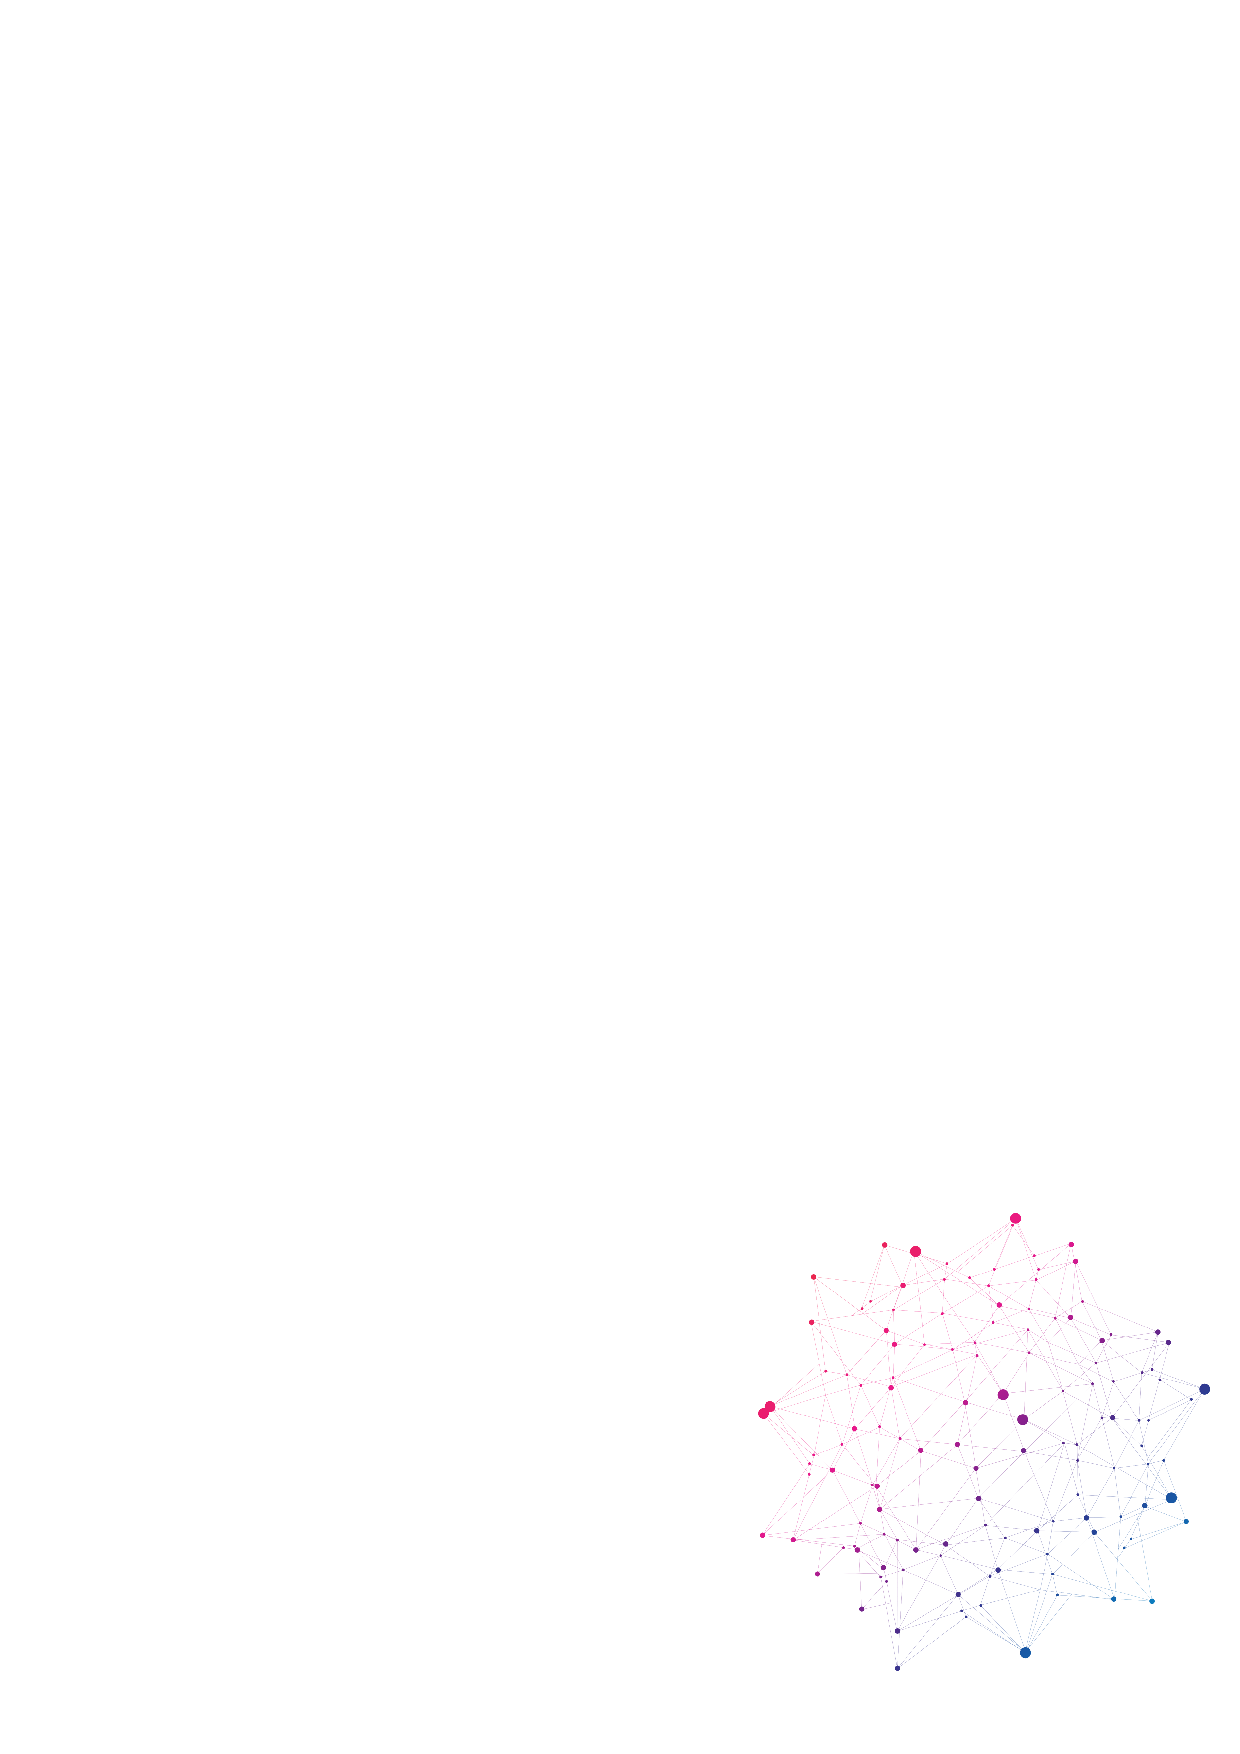
\includegraphics[width=\paperwidth]{Images/background.pdf}}
    \vspace*{1.2cm}
    \hspace*{1cm}{\Large Thank you!}\\
    \vspace*{0.6cm}
    \hspace*{1cm}{\Huge \alert{Any questions?}}
\end{frame}





\section{Extra}

\begin{frame}{Birth and death algorithm for updating the graph}

    \texttt{BDGraph} is an algorithm that follows a Birth-and-Death approach to decide whether to \alert{add} a new edge to the graph or \alert{delete} an already existing one.

    \pause
    
    % https://people.inf.ethz.ch/markusp/teaching/guides/guide-tables.pdf
    \begin{table}[tb]
        \centering
        \begin{tabular}{lcc}
        \toprule
        & Target distribution & B/D rates \\
        \hline
        \textbf{Before} & $P(\bm{G},\bm{K} \mid \bm{Y}) \propto P(\bm{Y} \mid \bm{K})P (\bm{K} \mid \bm{G})P(\bm{G})$ & $\cfrac{P(\bm{G}')}{P(\bm{G})}$ \\
        \textbf{After}  & $P(\bm{G},\bm{K} \mid \bm{Y}, \textcolor{sleekRed}{\bm{z}}) \propto P(\bm{Y} \mid \bm{K})P(\bm{K} \mid \bm{G})P(\bm{G} \mid \textcolor{sleekRed}{\bm{z}})$ & $\cfrac{P(\bm{G}' \mid \textcolor{sleekRed}{\bm{z}})}{P(\bm{G} \mid \textcolor{sleekRed}{\bm{z}})}$ \\
        \bottomrule
        \end{tabular}
    \end{table}
    where $\bm{G}' = \bm{G}^{\pm e}$ and $e$ is an edge.
    \pause
    \[
        \text{Birth rate} \propto \frac{P(\bm{G}^{+ e}\mid \bm{z})}{P(\bm{G}\mid \bm{z})} = \frac{S_{uv} + \alpha}{S^{\star}_{uv} + \beta}
        \quad
        \text{Death rate} \propto \frac{P(\bm{G}^{- e}\mid \bm{z})}{P(\bm{G}\mid \bm{z})} = \frac{S^{\star}_{uv} + \beta}{S_{uv} + \alpha}
    \]
    
\end{frame}

\begin{frame}{General steps for updating the partition}
    
    We perform an adaptive \alert{split and merge}.

    \fg{0.4}{Images/update_partition_splitmerge.pdf}
    \begin{enumerate}
        \item With probability $\alpha_{\text{split}}$, usually $0.5$, choose an \alert{split move}, otherwise a \alert{merge move}. Unless we are forced by extreme cases.
        \begin{enumerate}
            \item Propose a new partition by splitting one group into two or merging two adjacent, using two vectors of \alert{weights}, $\bm{a}^{(t)}$ and $\bm{d}^{(t)}$, to choose where to perform the move.
            \item Accept or reject using\vphantom{un banale} Metropolis Hastings. The target is:
            $f(\bm{z} \mid \bm{G}) \approx P(\bm{G} \mid \bm{z}) P(\bm{z})$
            \pause
            \begin{equation*}
                \alpha_{\text{accept}} = \min
                \bigg\{1,
                \overbrace{
                \underbrace{\frac{P(\bm{G} \mid \bm{z}')}{P(\bm{G} \mid \bm{z})}}_{\substack{\text{graph}\\\text{ratio}}}
                \underbrace{\frac{P(\bm{z}')}{P(\bm{z})}}_{\substack{\text{partition}\\\text{ratio}}}
                }^{\text{target ratio}}
                \underbrace{\frac{Q(\bm{z}',\bm{z})}{Q(\bm{z},\bm{z}')}}_{\substack{\text{proposal}\\\text{ratio}}}
                \bigg\}
            \end{equation*}
        \end{enumerate}
        
    \end{enumerate}

\end{frame}



\begin{frame}{Shuffle move}
    \begin{enumerate}
        \item[2.] To improve the mixing of the chain we also perform a \alert{shuffle move}.
            \begin{enumerate}
                \item[2.1] Propose a new partition by moving some nodes from a group to an adjacent one.
                \item[2.2] Accept or reject using Metropolis Hastings.
            \end{enumerate}

        \fg{0.4}{Images/update_partition_shuffle.pdf}
        \vspace*{0.5cm}
        \item[3.] The two weights vectors $\bm{a}^{(t)}$ and $\bm{d}^{(t)}$ are updated at each iteration $t$ as in \cite{bensonAdaptiveMCMCMultiple2018}.
    \end{enumerate}

\end{frame}



\begin{frame}{Adaptive step}
    The two weights vectors $\bm{a}^{(t)}$ and $\bm{d}^{(t)}$ are updated at each iteration $t$ as in \cite{bensonAdaptiveMCMCMultiple2018} using the following \textbf{adaptation scheme}.
    \pause
    
    \begin{itemize}
        \item If a \alert{split} move at node $i$ has been accepted, then update:
        \[
            \log (a_i^{(t+1)})=\log (a_i^{(t)})+\frac{h}{t/p}(\alpha_{\text{split}}-\alpha_{\text{target}}) .
        \]
        \item If a \alert{merge} move at node $i$ has been accepted, then update:
        \[
            \log (d_i^{(t+1)})=\log (d_i^{(t)})+\frac{h}{t/p}(\alpha_{\text{merge}}-\alpha_{\text{target}}) .
        \]
    \end{itemize}
Where $h>0$ is the initial adaptation, $t/p$ are the iterations $(t)$ per number of nodes $(p)$, $\alpha_{\text{target}}$ is the target MH acceptance rate and $\alpha_{\text{merge}} = 1 - \alpha_{\text{split}}$.
\end{frame}



\begin{frame}{Performance indexes: Kullback-Leibler}
    
    Suppose that we have two multivariate normal distributions, with means $\mu_0, \mu_1$ and with (non-singular) covariance matrices $\Sigma_0, \Sigma_1$. If the two distributions have the same dimension, $k$, then the relative entropy between the distributions is as follows:
    \[
        D_{\mathrm{KL}}\left(\mathcal{N}_0 \| \mathcal{N}_1\right)=\frac{1}{2}\left(\operatorname{tr}\left(\Sigma_1^{-1} \Sigma_0\right)-k+\left(\mu_1-\mu_0\right)^{\top} \Sigma_1^{-1}\left(\mu_1-\mu_0\right)+\ln \left(\frac{\operatorname{det} \Sigma_1}{\operatorname{det} \Sigma_0}\right)\right)
    \]
\end{frame}


\begin{frame}{Performance indexes: Rand index}
    Given a set of $n$ elements $S=\left\{o_1, \ldots, o_n\right\}$ and two partitions of $S$ to compare, $X=\left\{X_1, \ldots, X_r\right\}$, a partition of $S$ into $r$ subsets, and $Y=\left\{Y_1, \ldots, Y_s\right\}$, a partition of $S$ into $s$ subsets, define the following:
    \begin{itemize}
        \item $a$, the number of pairs of elements in $S$ that are in the same subset in $X$ and in the same subset in $Y$
        \item $b$, the number of pairs of elements in $S$ that are in different subsets in $X$ and in different subsets in $Y$
        \item c, the number of pairs of elements in $S$ that are in the same subset in $X$ and in different subsets in $Y$
        \item $d$, the number of pairs of elements in $S$ that are in different subsets in $X$ and in the same subset in $Y$
    \end{itemize}
    The Rand index, $R$, is:
    \[
    R=\frac{a+b}{a+b+c+d}=\frac{a+b}{\binom{n}{2}}
    \]
    %Intuitively, $a+b$ can be considered as the number of agreements between $X$ and $Y$ and $c+d$ as the number of disagreements between $X$ and $Y$.
\end{frame}





\begin{frame}{Performance indexes: BFDR}
    
    Given the estimated p-links matrix $\hat{p}_{j k}$ the Bayesian False Discovery rate is
    \[
        \operatorname{BFDR}(s)=\frac{\sum_{j<k}\left(1-\hat{p}_{j k}\right) \mathbbm{1}_{\left(\hat{p}_{j k} \geq s\right)}}{\sum_{j<k} \mathbbm{1}_{\left(\hat{p}_{j k} \geq s\right)}}
    \]
    and the threshold $s$ is selected so that BFDR is below $0.05$.
\end{frame}